\documentclass[10pt, letterpaper]{article}
\usepackage[utf8]{inputenc}
\usepackage{amsmath}
\usepackage{amssymb}
\usepackage{bbm}
\usepackage{booktabs}
\usepackage{caption}
\usepackage{color}
\usepackage[shortlabels]{enumitem}
\usepackage{fancyhdr}
\usepackage{hyperref}
\usepackage{geometry}
\geometry{a4paper,scale=0.8}
\usepackage{graphicx}
\graphicspath{ {./img/}}
\usepackage{listings}
\usepackage{mathtools}
\usepackage{mathrsfs}
\usepackage{setspace}
\usepackage{subfigure}
\renewcommand{\baselinestretch}{1.3}

% set-up header & footer
\pagestyle{empty}
\fancyhf{}
\cfoot{\thepage}
\lhead{%
\textbf{University of California, Berkeley} \\
Department of Civil \& Environ. Eng.
}
\rhead{\textbf{CS 285 Deep Reinforcement Learning}\\\date{\today}}

\title{%
    \textbf{Homework 5}
}
\author{Juanwu Lu (3037432593)\\ \small(M.Sc. Civil Engineering, UC Berkeley)}
\date{}

% set-up code listing
\definecolor{dkgreen}{rgb}{0,0.6,0}
\definecolor{gray}{rgb}{0.5,0.5,0.5}
\definecolor{manuve}{rgb}{0.58,0,0.82}

\lstset{frame=tb,
    language=Python,
    aboveskip=3mm,
    belowskip=3mm,
    showstringspaces=false,
    columns=flexible,
    basicstyle={\small\ttfamily},
    numbers=none,
    numberstyle=\tiny\color{gray},
    keywordstyle=\color{blue},
    commentstyle=\color{dkgreen},
    stringstyle=\color{manuve},
    breaklines=true,
    breakatwhitespace=true,
    tabsize=3
}

\begin{document}
\maketitle
\captionsetup[figure]{labelfont={bf},labelformat={default},labelsep=period,name={Figure}}
\captionsetup[table]{labelfont={bf},labelformat={default},labelsep=period,name={TABLE}}
\thispagestyle{fancy}
\pagestyle{plain}

% Problem 1
\section*{Problem 1 "Unsupervised" RND and exploration performance}
\subsection*{Part 1 Results}

\begin{figure}[h!]
    \centering
    \subfigure[]{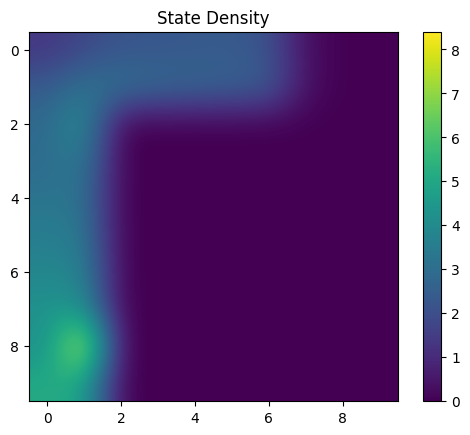
\includegraphics[width=0.35\textwidth]{q1_easy_random.png}}
    \subfigure[]{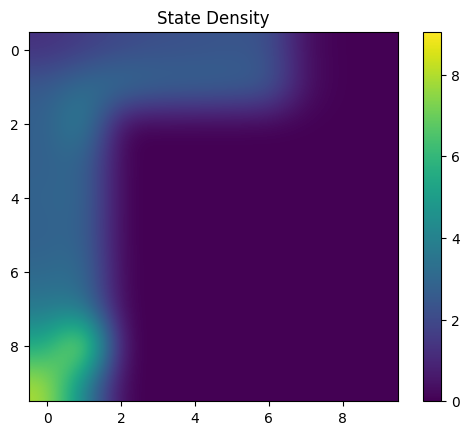
\includegraphics[width=0.35\textwidth]{q1_easy_rnd.png}}
    \caption{Results from PointmassEasy Environment: (a) Random exploration with epsilon-greedy; (b) Exploration with RND. State density of from the two algorithms are similar but RND unexpectedly has a denser density around the lower left corner (origin).}
    \label{fig:1}
\end{figure}

\begin{figure}[h!]
    \centering
    \subfigure[]{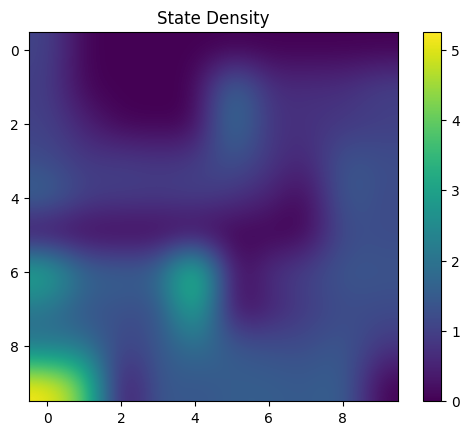
\includegraphics[width=0.35\textwidth]{q1_medium_random.png}}
    \subfigure[]{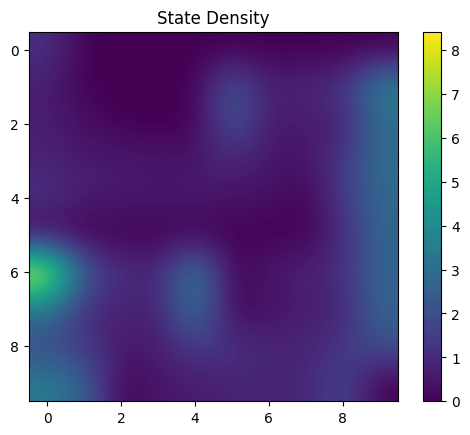
\includegraphics[width=0.35\textwidth]{q1_medium_rnd.png}}
    \caption{Results from PointmassMedium Environment: (a) Random exploration with epsilon-greedy; (b) Exploration with RND. State density of from the two algorithms are similar but RND has a more uniformly distributed density than the random exploration one.}
    \label{fig:2}
\end{figure}

\begin{figure}[h!]
    \centering
    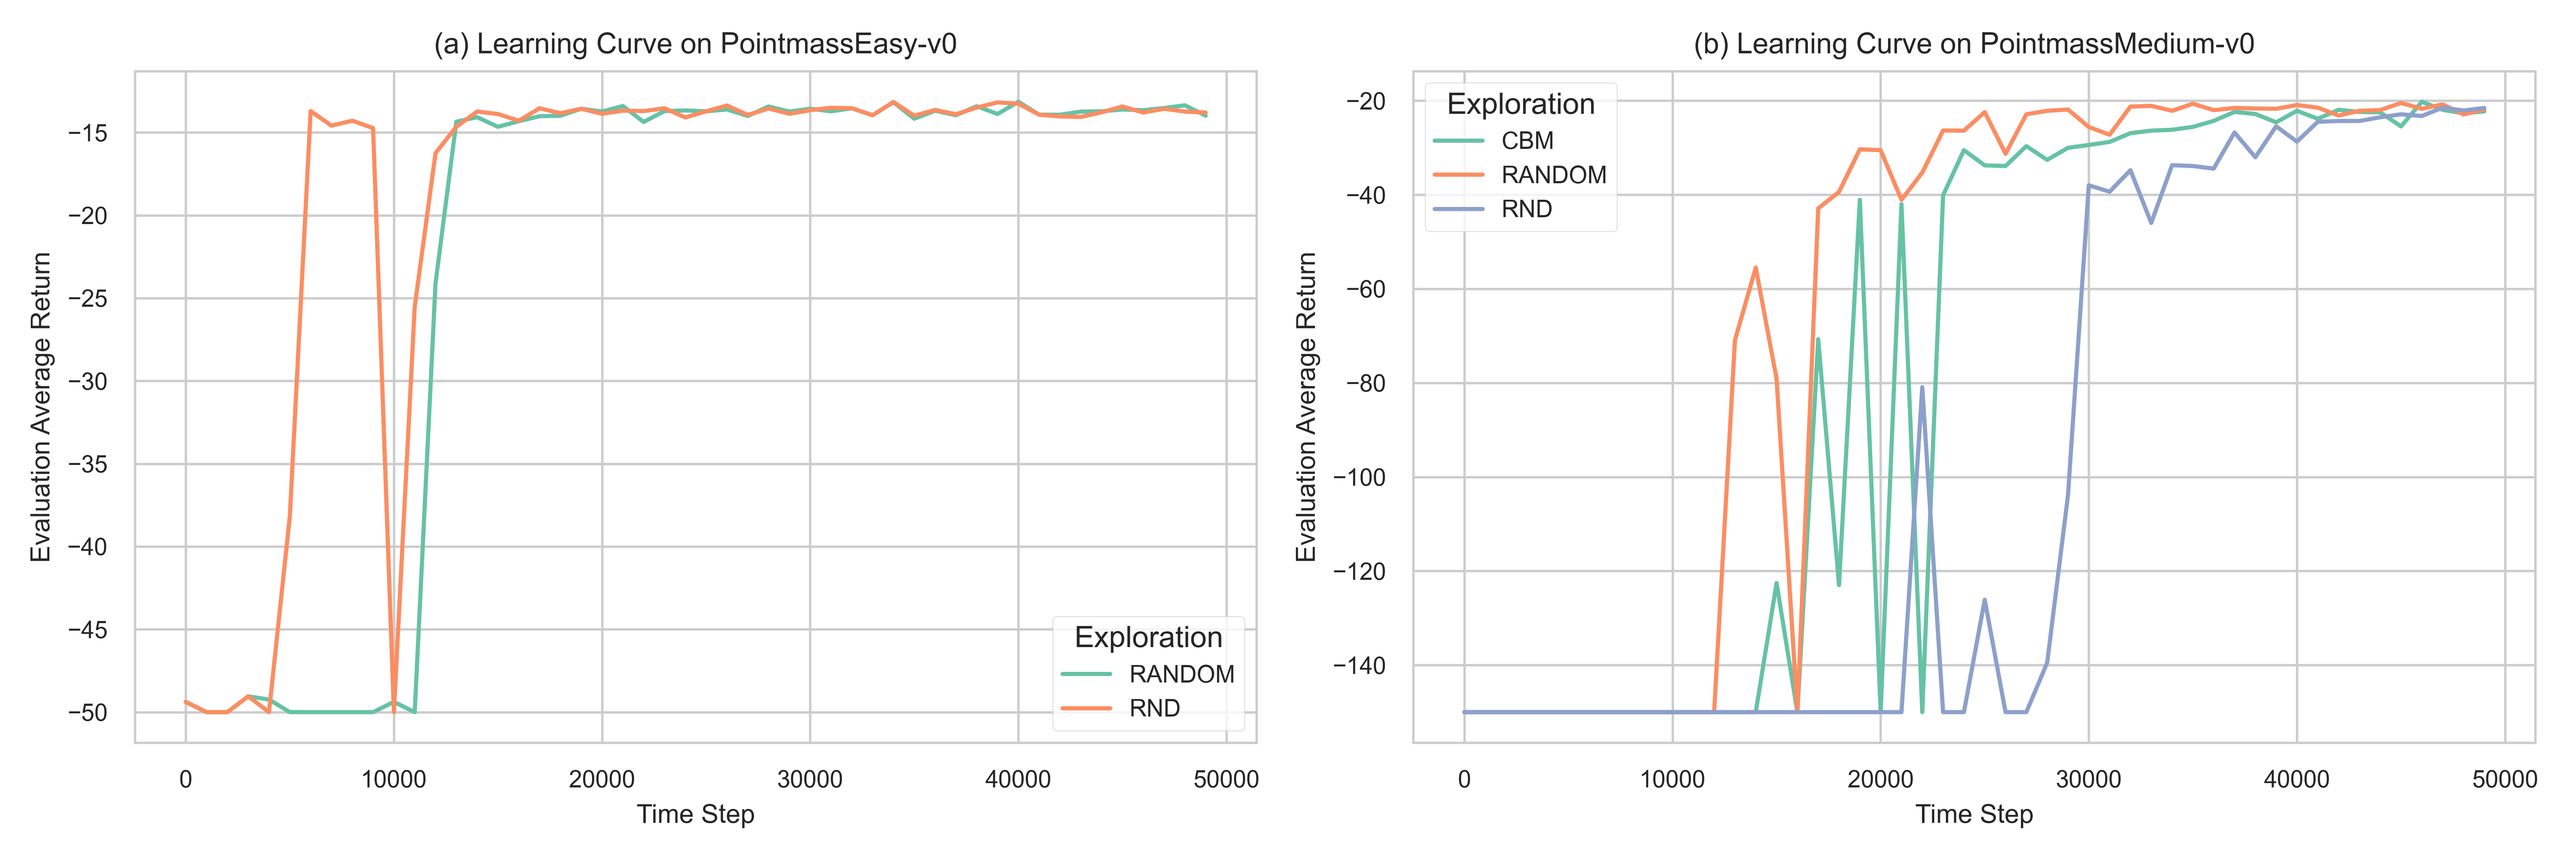
\includegraphics[width=\textwidth]{q1_learning_curve.png}
    \caption{Learning curve from the two environments. RND reaches higher score faster than epsilon-greedy on the PointmassEasy environment, while slower on the PointmassMedium environment.}
    \label{fig: 3}
\end{figure}

\subsection*{Part 2 Results}

\pagebreak
\section*{Problem 2 Offline learning on exploration data}
\subsection*{Part 1 Compare CQL to DQN on the \texttt{medium} environment}

\subsection*{Part 2 Ablation study on amount of exploration data}

\subsection*{Part 3 Ablation study on the regularizer weight $\alpha$}

\pagebreak
\section*{Problem 3 "Supervised" exploration with mixed reward bonuses}

\pagebreak
\section*{Problem 4 Offline Learning with AWAC}

\begin{figure}[h!]
    \centering
    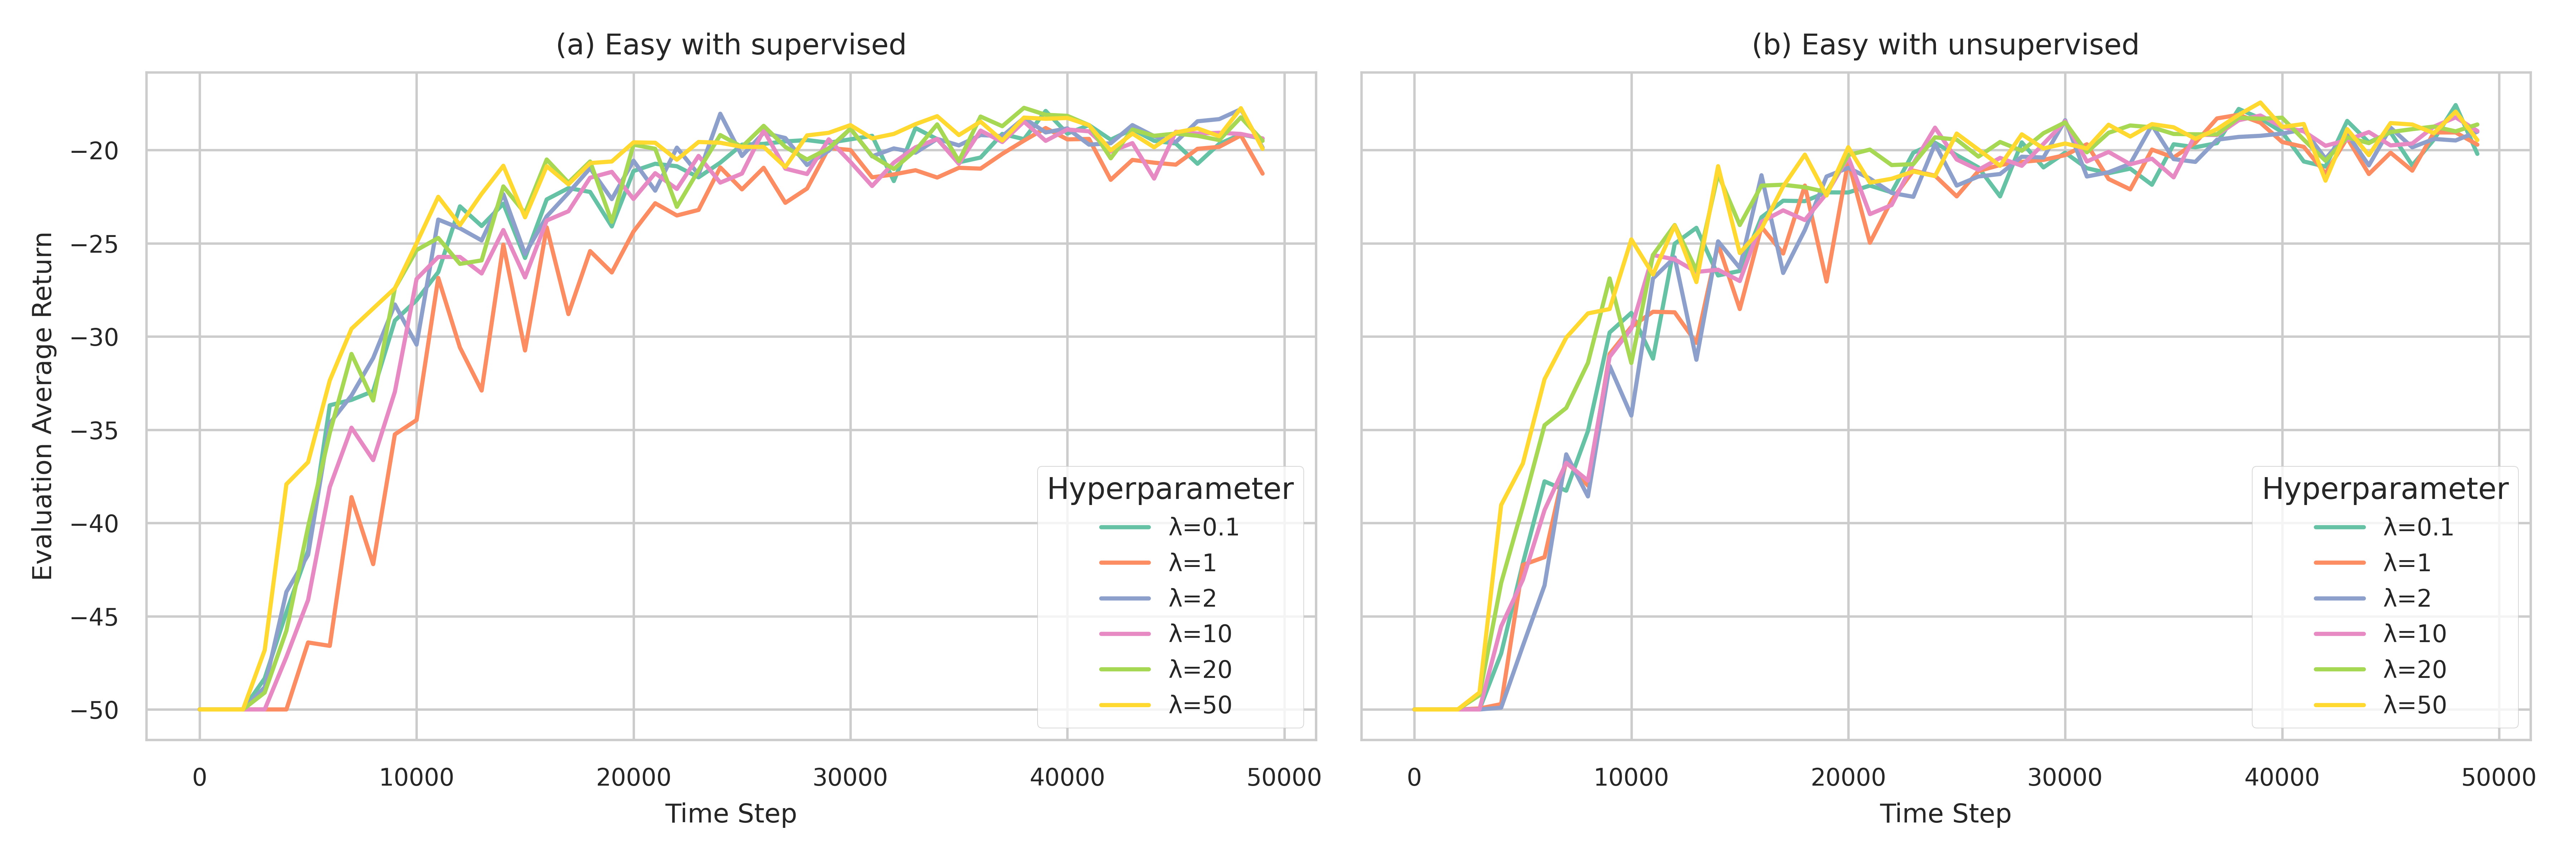
\includegraphics[width=\textwidth]{q4_easy.png}
    \caption{Learning curve from \texttt{PointmassEasy} environment: (a) supervised algorithm with different $\lambda$ settings; (b) unsupervised algorithm with different $\lambda$ settings. Explorations with supervised and unsupervised perform quite similar in this environment, which I think is partly due to the simplicity of the task.}
\end{figure}

\begin{figure}[h!]
    \centering
    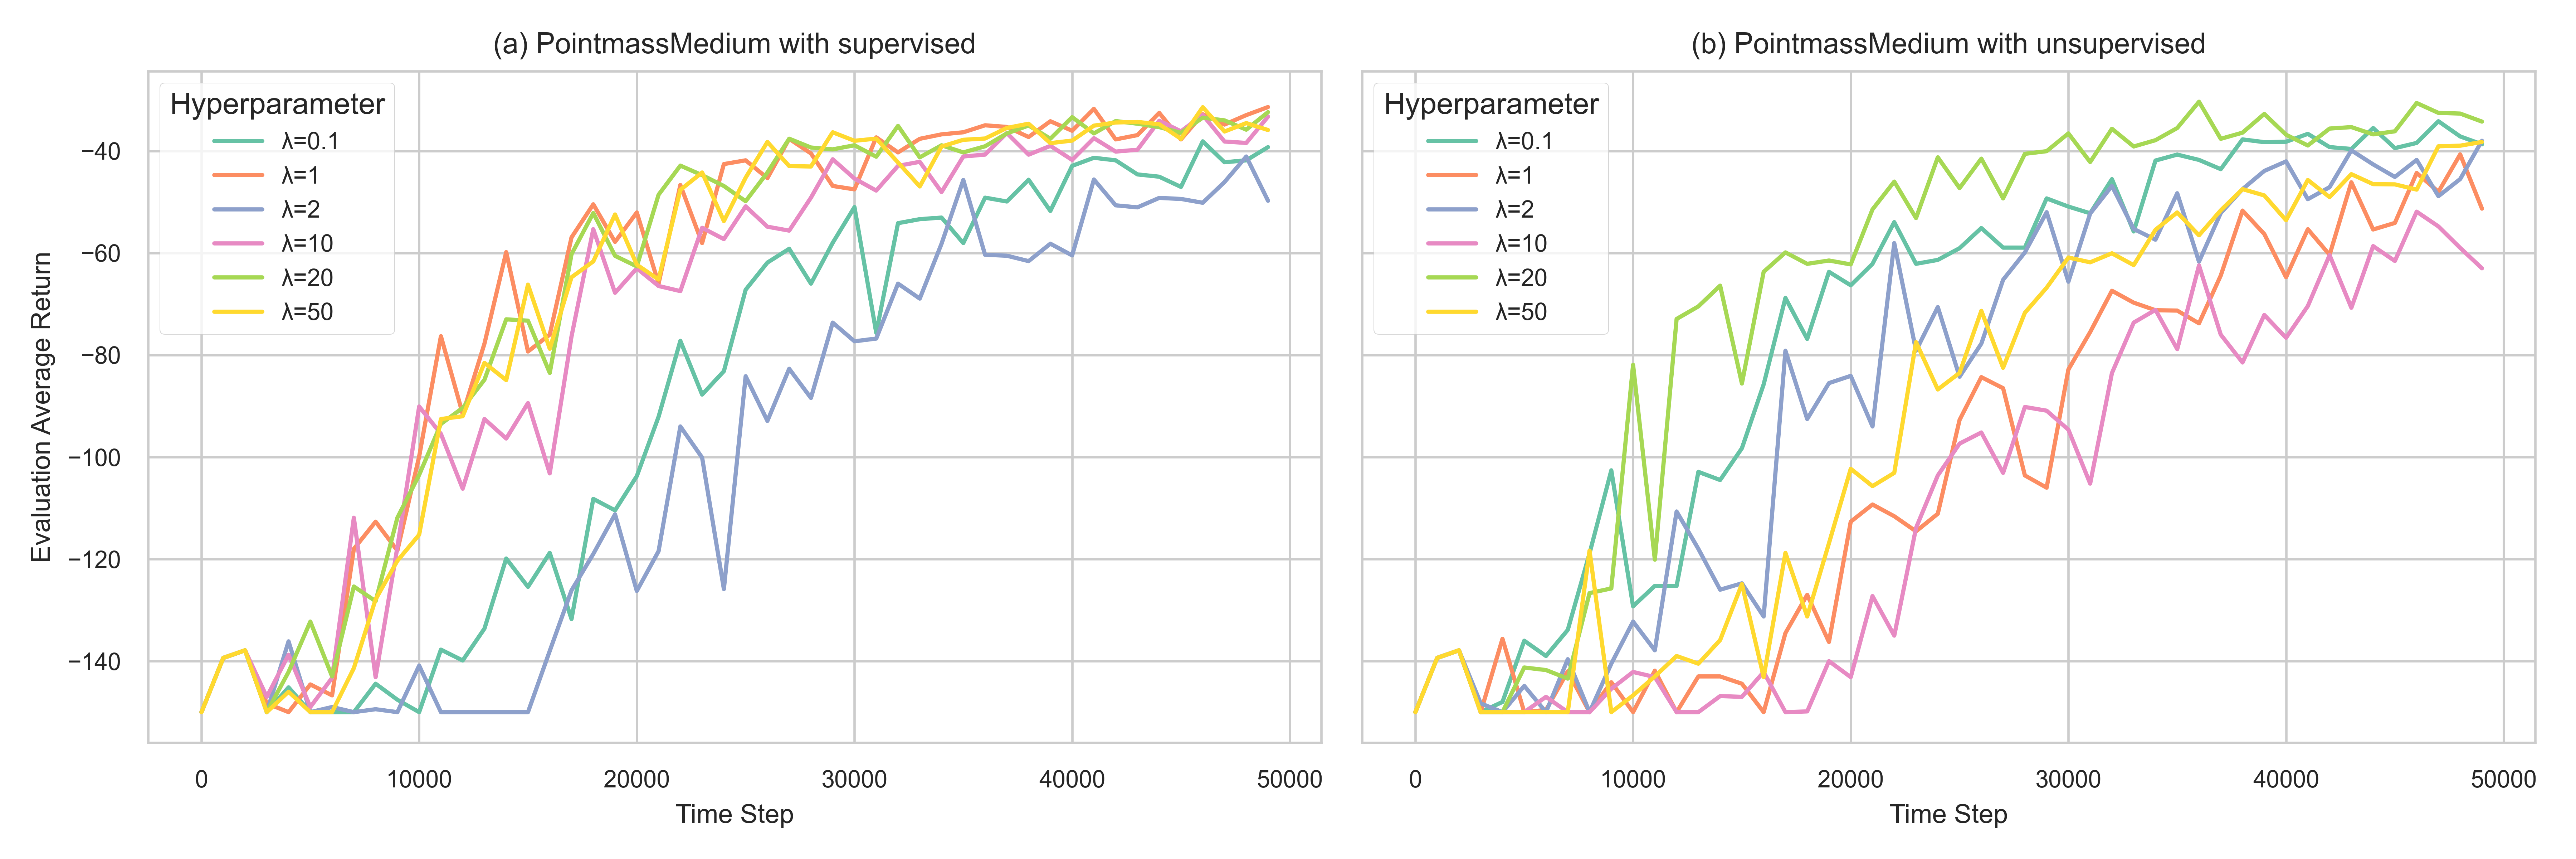
\includegraphics[width=\textwidth]{q4_medium.png}
    \caption{Learning curve from \texttt{PointmassMedium} environment: (a) supervised algorithm with different $\lambda$ settings; (b) unsupervised algorithm with different $\lambda$ settings. Unexpectedly, explorations with unsupervised perform a bit better overall in this environment with faster reaching a higher return. The best $\lambda$ setting for supervised and unsupervised RND are $\lambda=20$ and $\lambda=0.1$, respectively.}
\end{figure}

\pagebreak
\section*{Problem 5 Offline Learning with IQL}


\end{document}